\ifthenelse{\boolean{plosone}}{
  \begin{figure*}
  \begin{adjustwidth}{-2.25in}{0in} % Comment out/remove adjustwidth environment i
}{
  \begin{table*}
}
\begin{boxedminipage}{\linewidth}
\section*{Relational algebra}

Relational operators operate on existing relations to produce \emph{derived} relations for answering a wide variety of specific queries.
These operators do not retrieve any data from the database until the resulting expression is used to \emph{fetch} the data.
Relational operators are based on the concept of \emph{matching tuples}: 
Two tuples are considered matching  \emph{unless} they share an attribute with the same name but different values.

\subsection*{Restriction:  {\sf A \& B}, {\sf A -- B}}
The restriction A\&B denotes a relation comprising all tuples from A that match any tuple in {\sf B}.  

\begin{center}
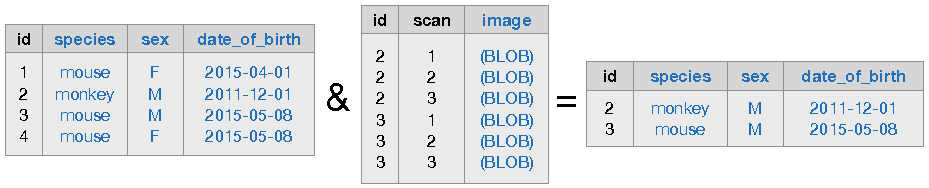
\includegraphics{./figures/restriction.pdf}
\end{center}

The inverse restriction {\sf A--B} denotes all tuples from {\sf A} that do not match any tuple in {\sf B}.

\begin{center}
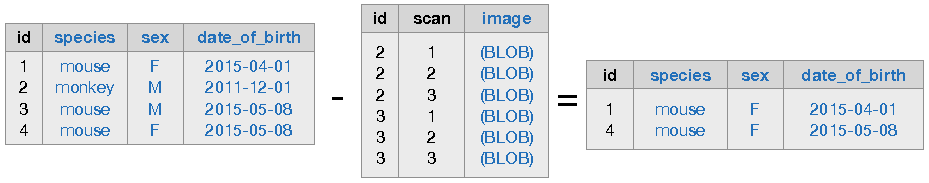
\includegraphics{./figures/antijoin.pdf}
\end{center}


\subsection*{Join: {\sf A * B}}
The join {\sf A*B} is the set of all tuples that can be produced by merging matching tuples from {\sf A} and {\sf B}:

\begin{center}
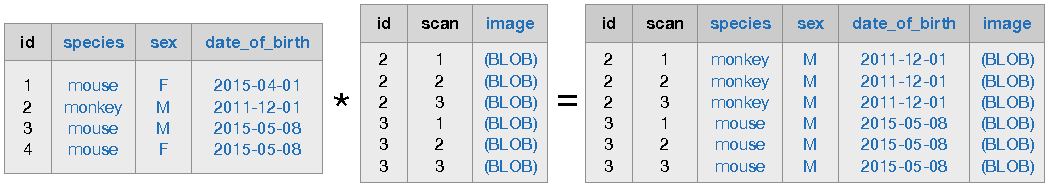
\includegraphics{./figures/join.pdf}
\end{center}
All attributes in {\sf A} and {\sf B} that share the same names must belong to the primary key in either relation.

\subsection*{Projection: {\sf A.pro(attributes)}}
The projection {\sf A.pro(attributes)} modifies the heading of {\sf A} by selecting a subset of its attributes (project), renaming attributes (rename), computing new attributes (expand), and computing summary statistics from other relations (aggregate).
The primary key attributes cannot be excluded from the resulting relation but may be renamed. 

\begin{center}
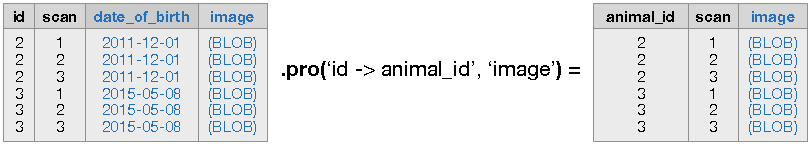
\includegraphics{./figures/project.pdf}
\end{center}

Please refer to the online documentation for more detailed descriptions.
\end{boxedminipage}
\caption{Relational operators of DataJoint}
\label{algebra}
\ifthenelse{\boolean{plosone}}{
  \end{adjustwidth}
  \end{figure*}
}{
  \end{table*}
}
